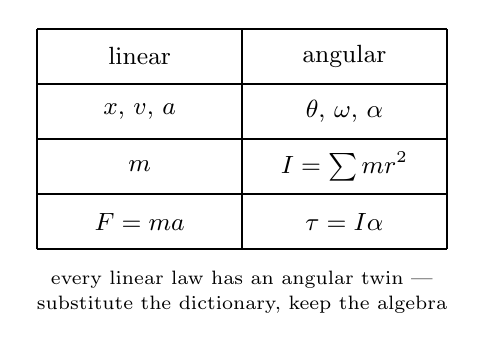
\begin{tikzpicture}[font=\small]
\draw[thick] (0,0) grid[xstep=2.6,ystep=0.7] (5.2,2.8);
\node at (1.3,2.45) {linear};\node at (3.9,2.45) {angular};
\node at (1.3,1.75) {$x$, $v$, $a$};\node at (3.9,1.75) {$\theta$, $\omega$, $\alpha$};
\node at (1.3,1.05) {$m$};\node at (3.9,1.05) {$I=\sum mr^{2}$};
\node at (1.3,0.35) {$F=ma$};\node at (3.9,0.35) {$\tau=I\alpha$};
\node[align=center] at (2.6,-0.55) {\scriptsize every linear law has an angular twin ---\\[-2pt]\scriptsize substitute the dictionary, keep the algebra};
\end{tikzpicture}
